	The Lotka-Volterra model 
\begin{align} %\label{eqn:DeterministicLotkaVolterra}
	\frac{dx}{dt} &= ax - bxy, \label{eqn:DetLotkaVolterraArnoldA}
	\\
	\frac{dy}{dt} &=-by +dxy,\label{eqn:DetLotkaVolterraArnoldB}
\end{align}
describes in a very simple way, the interaction of two populations. Usually, $x$, $y$, represent
the predator and prey populations, respectively. The linear terms $ax$, $-by$, describes the behavior
of a specie in the absence of the other, and the quadratic terms describes the interaction. 
Although this model has been criticized for being unrealistic, its simplicity permits
understand essential features of the predator-prey interaction \cite{may2001stability}. 

	For positive initial conditions,
all solutions, except the fixed-point $(\bar{x}, \bar{y})=(b/d, a/b)$, are periodic. However, the standard
procedures to form finite-difference schemes generally give numerical solutions that spiral into or away from the 
fixed-point. Mickens' \cite{Mickens2003} and Serghini's \cite{SerghiniMounim2004} methods, produce solutions that are 
periodic, being the 
second more precise. So, we compare the performance of the deterministic \SM method with 
these non-standard schemes see \Cref{fig:DeterministicLotkaVolterra}.
%\Cref{fig:DetPhasePotraitLotkaVolterraArnold},
%\Cref{subfig:DetX1LotkaVolterraArnold},
%\Cref{subfig:DetX2LotkaVolterraArnold}.

	However, in any real ecosystem are two sources of fluctuation \cite{may2001stability}:
\begin{inparaenum}[(i)]
	\item
		The population are finite and discrete, that is, its size change in integral steps. This
		is called demographic stochasticity or internal fluctuations.
	\item
		A realistic biological environment is not deterministic. Consequently, a better description
		should consider fluctuation in the phenomenological parameters like, growth rates, carrying capacities, etc.
		This kind of fluctuations is called external.
\end{inparaenum}

	Since the contribution of internal fluctuations decrease with the size of the population, usually, stochastic
models add randomness in the environmental parameters, see for example 
\cite{Bahar2004, Mao2002, Mao2003, Mao2009, Takeuchi2006, Rudnicki2007, Liu2013d, Yagi2011}. 
We consider the stochastic Lotka-Volterra model studied in \citet{Arnold1979}. 
Here, the authors suppose that the environmental fluctuations will mainly manifest in the growth rate $a$ with
$a\to a+\sigma dW_t$, where $a$ represents the mean grow rate and $\sigma^2$ controls the intensity of the 
white noise $dB(t)$. So, they obtain the following SDE:
\begin{align}
	dX^{(1)}_t &= X^{(1)}_t(a -b X^{(2)}_t) dt +\sigma X^{(1)}_t dW_t
	\label{eqn:StoLotkaVolterraArnold1} \\
	dX^{(2)}_t &= X^{(2)}_t( X^{(1)}_t - d).
	\label{eqn:StoLotkaVolterraArnold2}
\end{align}
With this on mind, taking
\begin{align*}
	a_1(x_k, y_k) &:= a - b y_k, & b_1(y_k):= 0,\\
	a_2(x_{k+1}, y_k) &:= b x_{k+1} -d, & b_2(y_k):= 0,
\end{align*}
in \eqref{eqn:SteklovSchem2}, we get the \SM method
\begin{align}
	X^{(1)}_{k+1} &= \exp \left[ a_1 \left( X^{(1)}_k,X^{(2)}_k \right) h \right] X^{(1)}_k 
		+\sigma X^{(1)}_k \Delta 	W_k,  \notag \\
%
	X^{(2)}_{k+1} &= \exp \left[ a_2\left(X^{(1)}_{k+1},X^{(2)}_k\right) h \right] X^{(2)}_k, \\
		a_1\left( X^{(1)}_k, X^{(2)}_k \right) &:= a - b X^{(2)}_k, \qquad
		a_2\left( X^{(1)}_{k+1}, X^{(2)}_k \right):= b X^{(1)}_{k+1} -d. \notag
\end{align}
In 
	\Cref{subfig:StoPhasePotraitLotkaVolterraArnold},
	\Cref{subfig:StoX1LotkaVolterraArnold}, and
	\Cref{subfig:StoX2LotkaVolterraArnold}
we compare the noisy trajectories produced with this scheme and the EM.

\begin{figure}[tb]
	\centering
	\subfloat[]{
		
		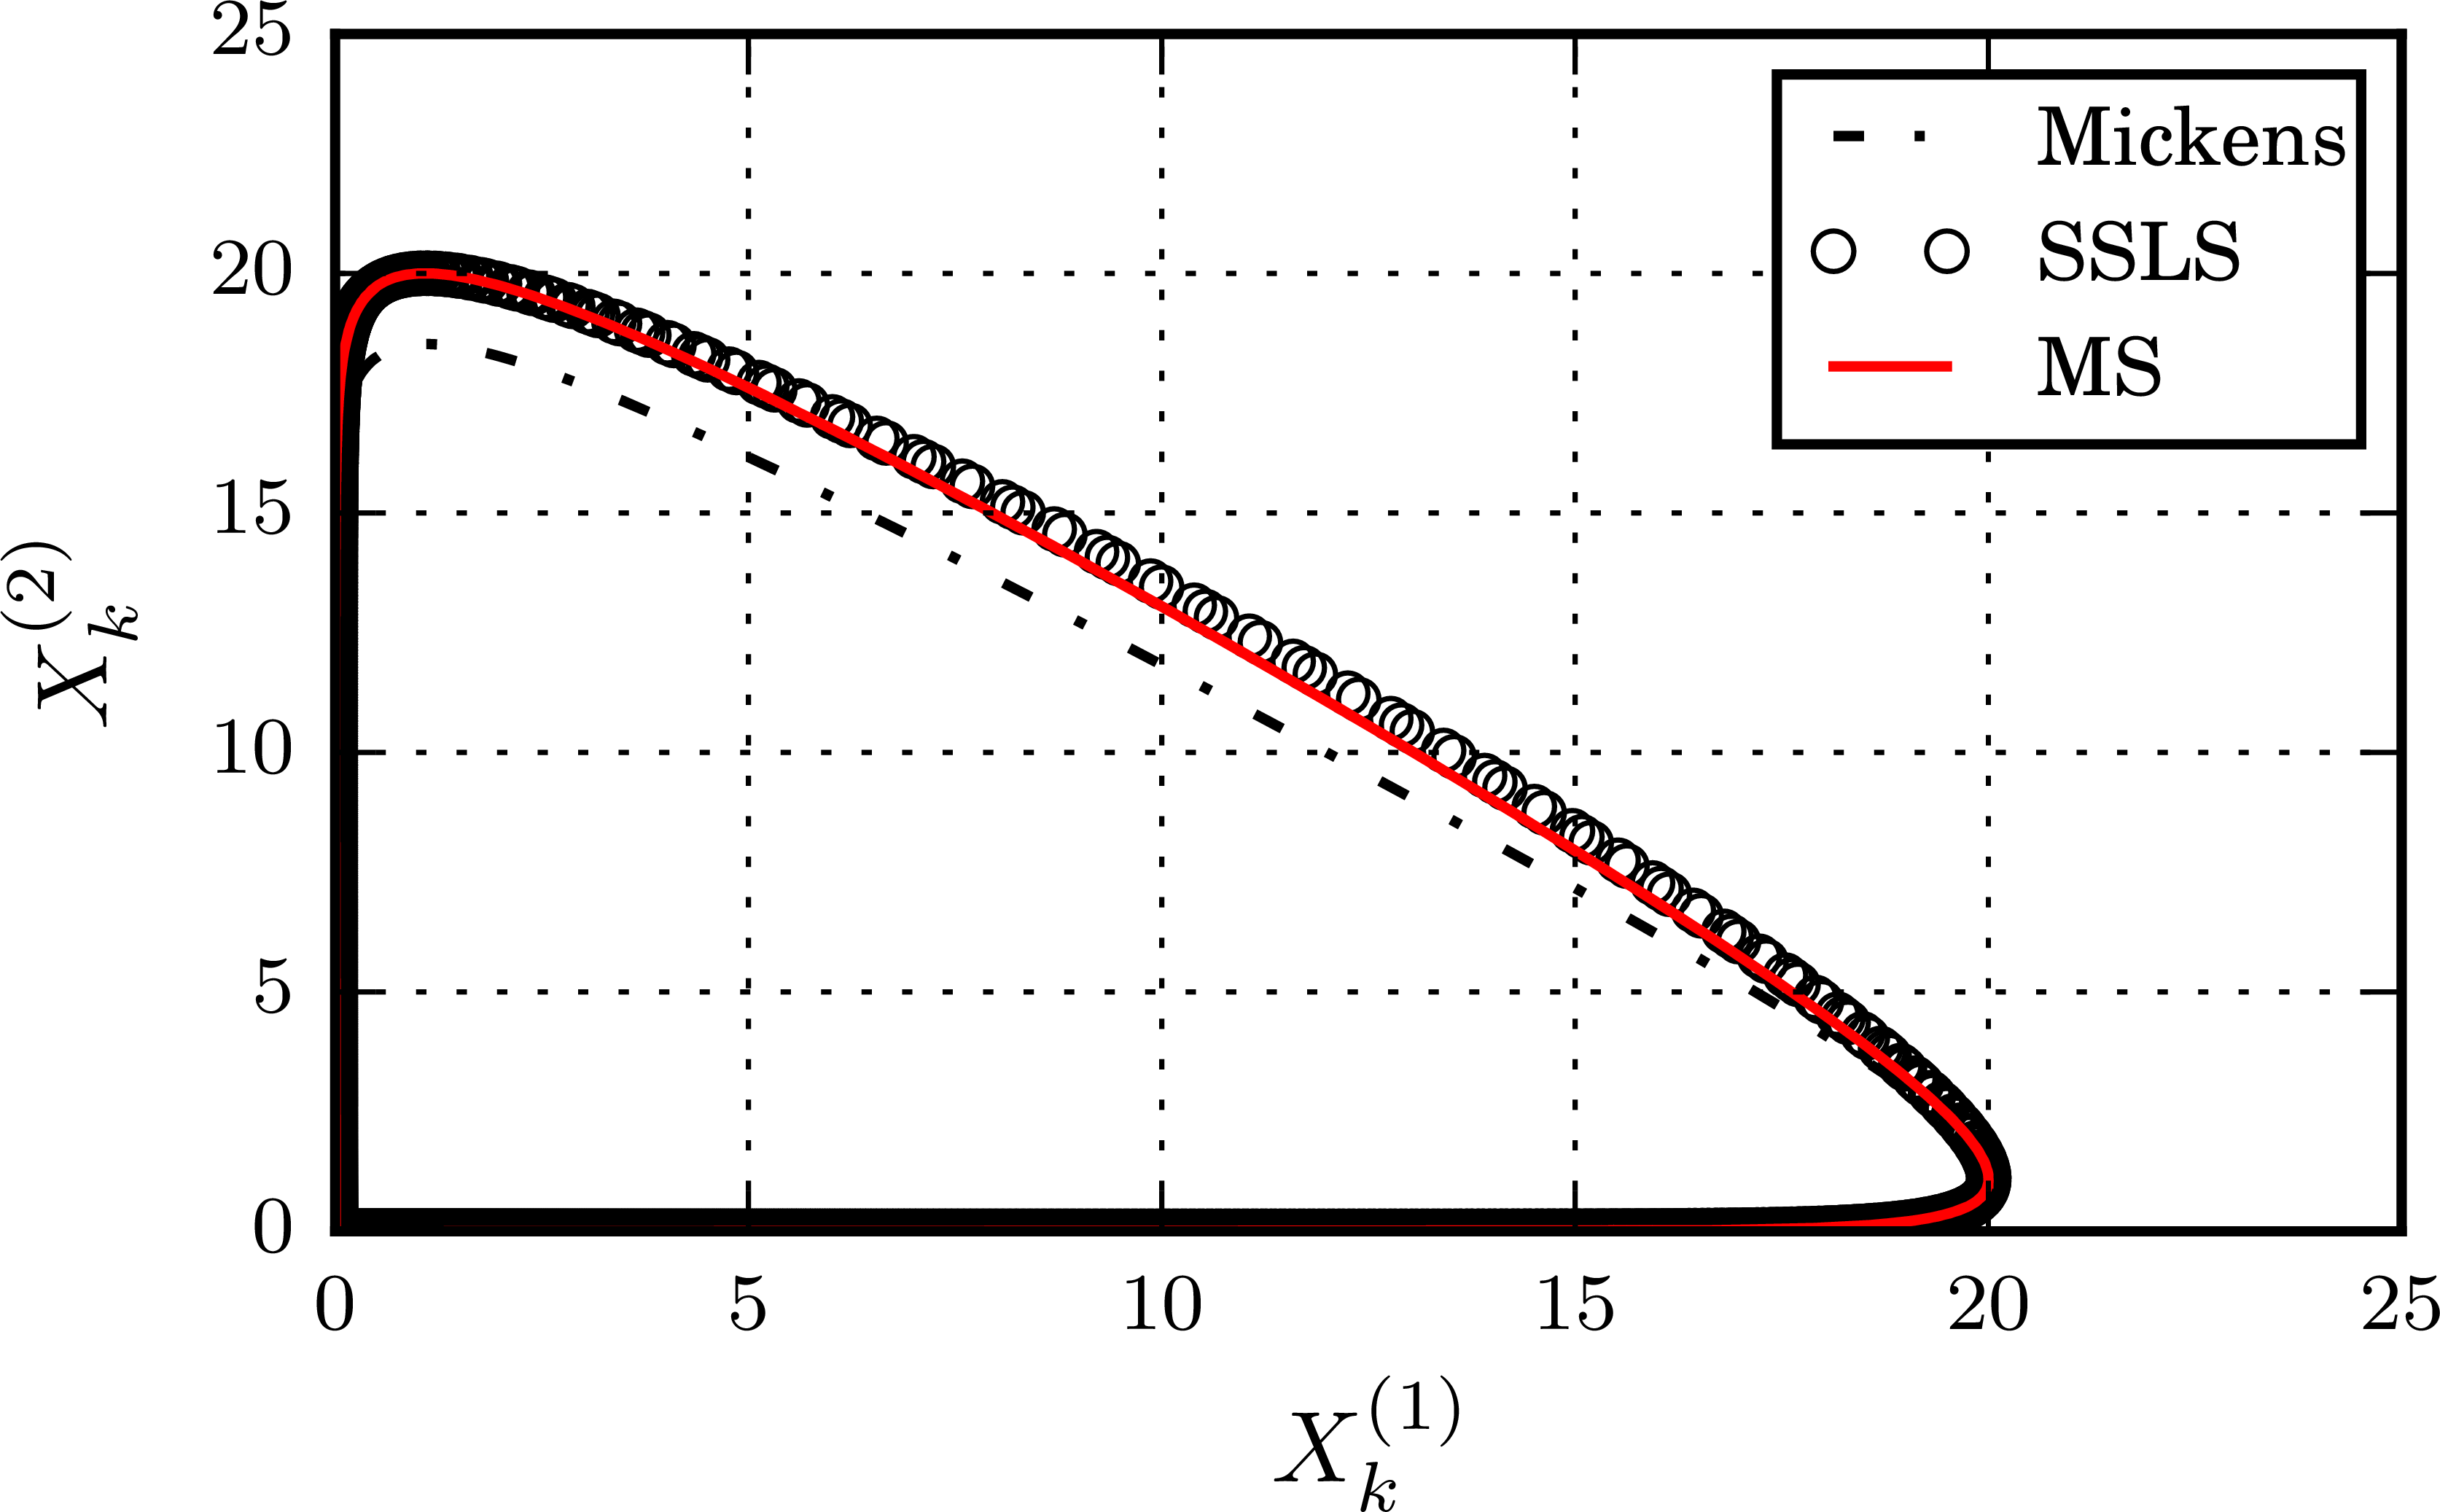
\includegraphics{./papers/paperB/figures/DetPhasePotraitLotkaVolterraArnold.png}
		\label{fig:DetPhasePotraitLotkaVolterraArnold}
	} \\
	\subfloat[]{
		\centering
		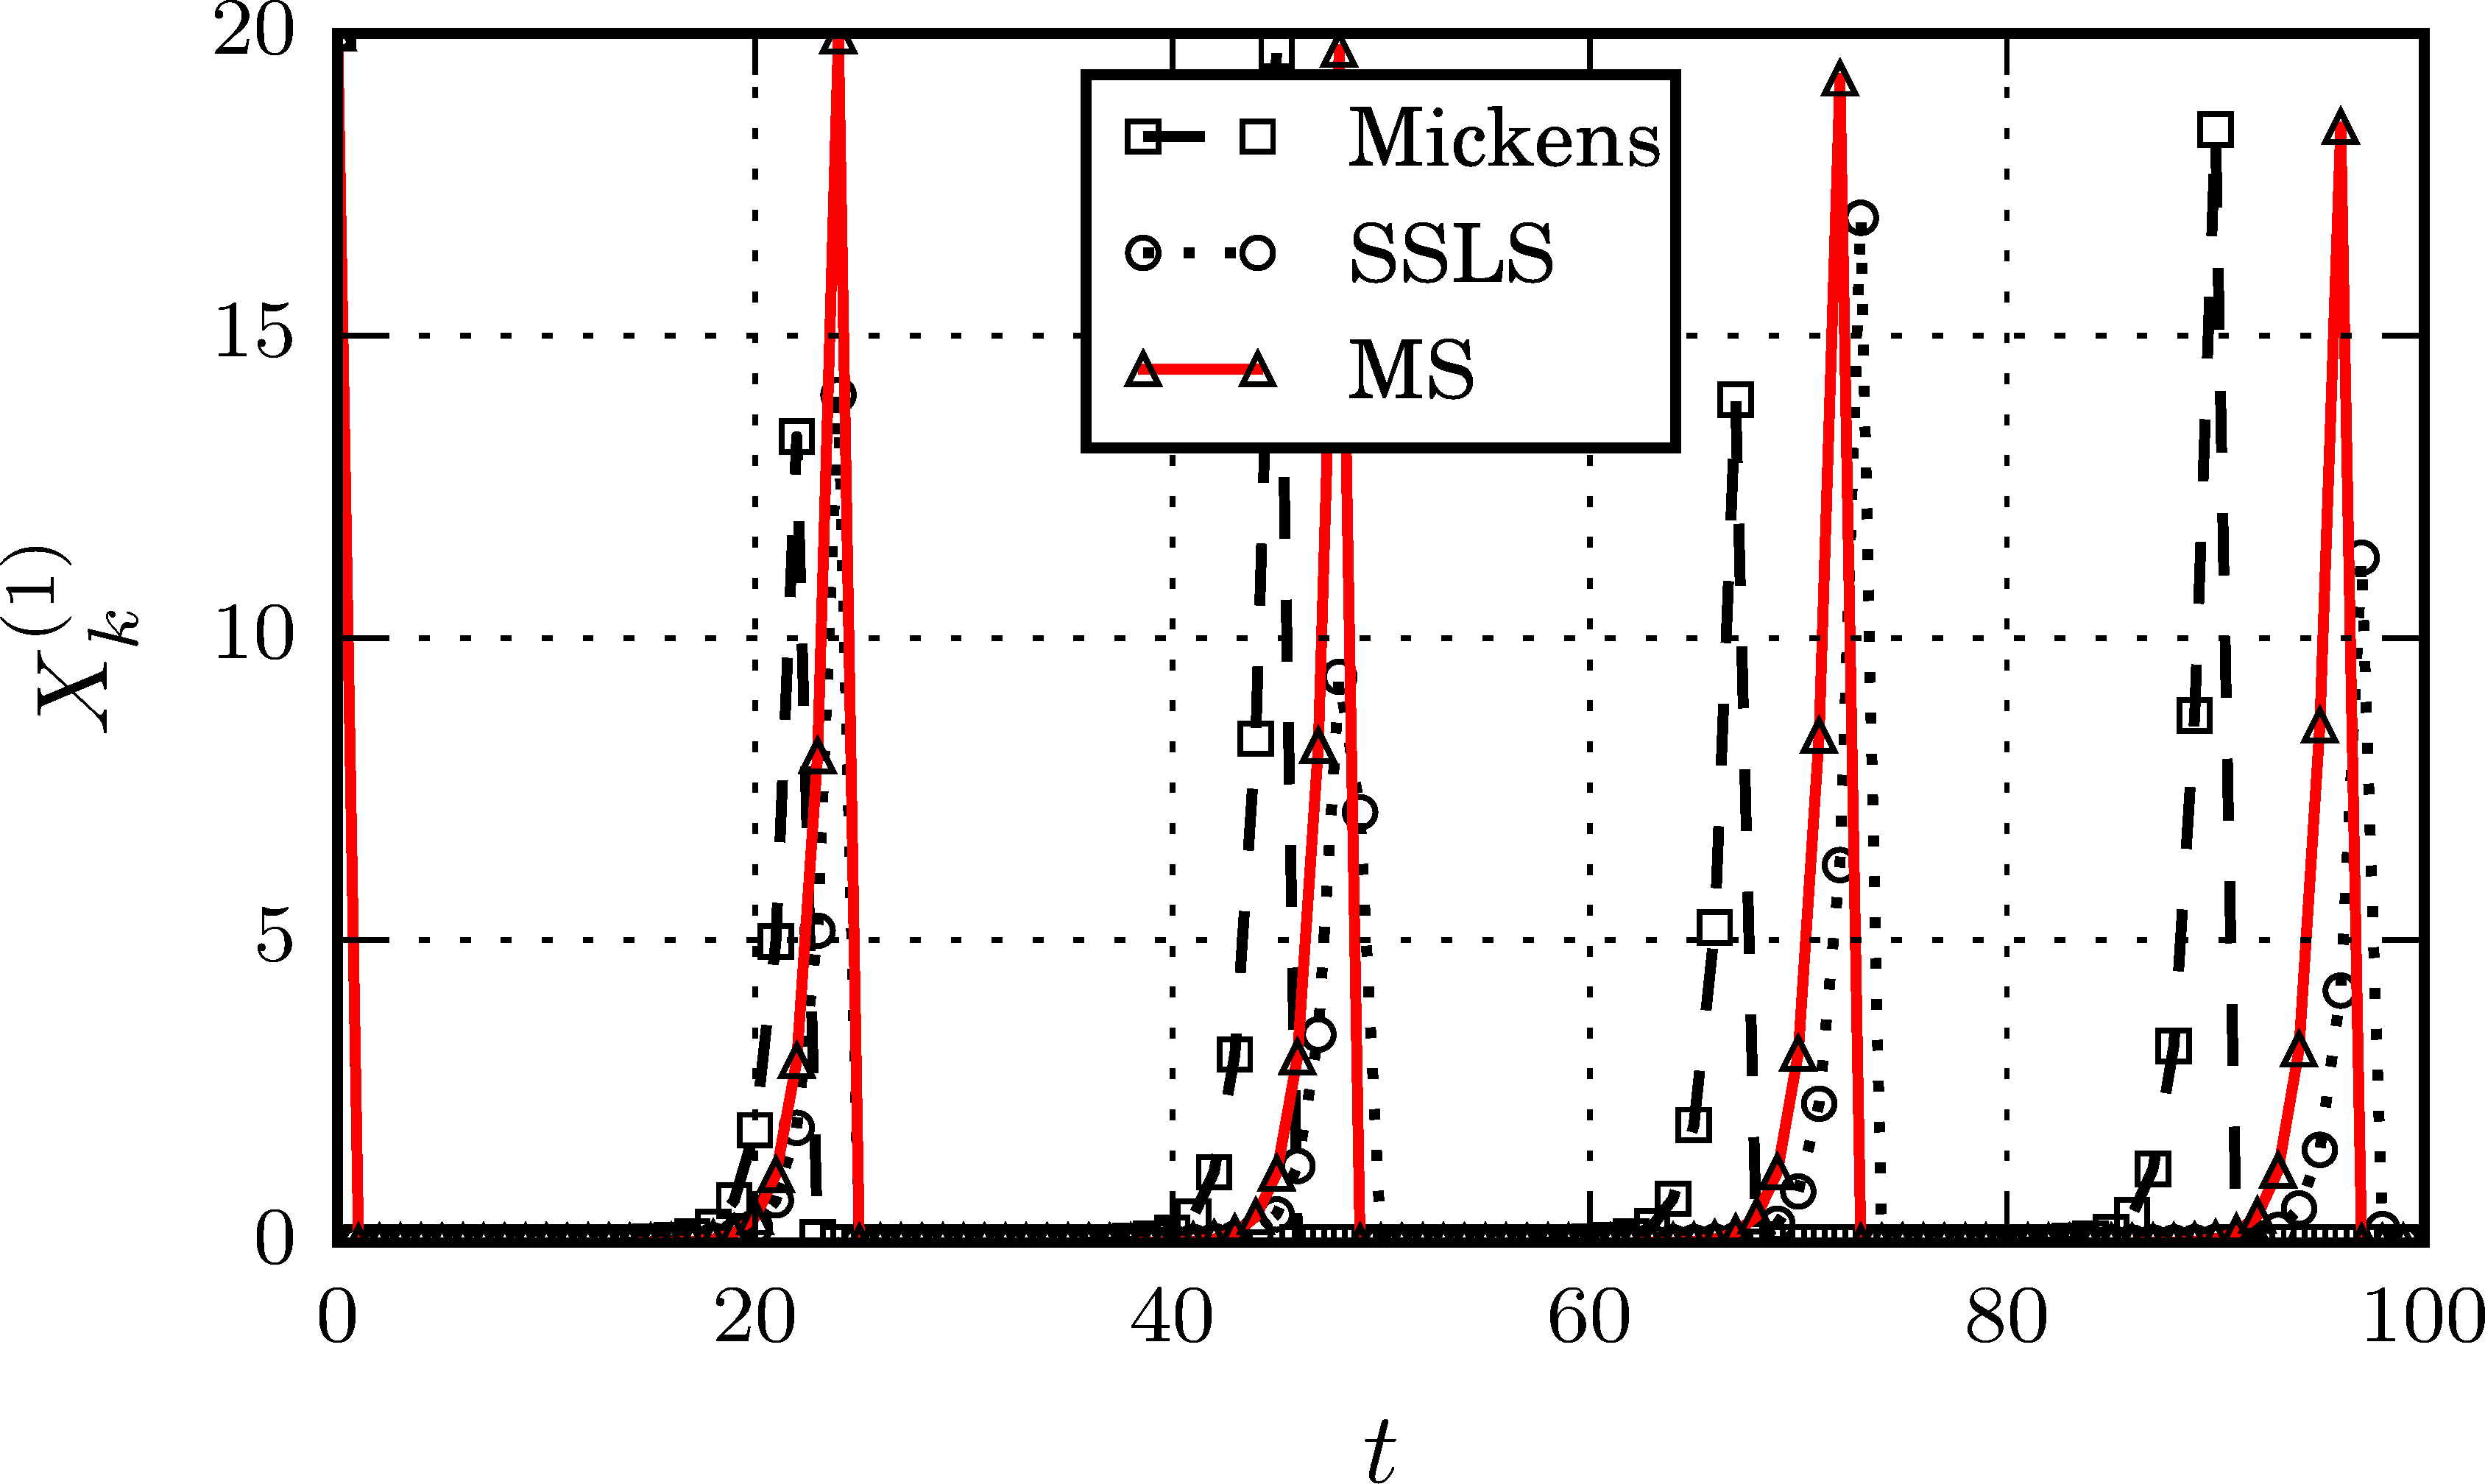
\includegraphics{./papers/paperB/figures/DetX1LotkaVolterraArnold.png}
		\label{subfig:DetX1LotkaVolterraArnold}
		}
	\subfloat[]{
		\centering
		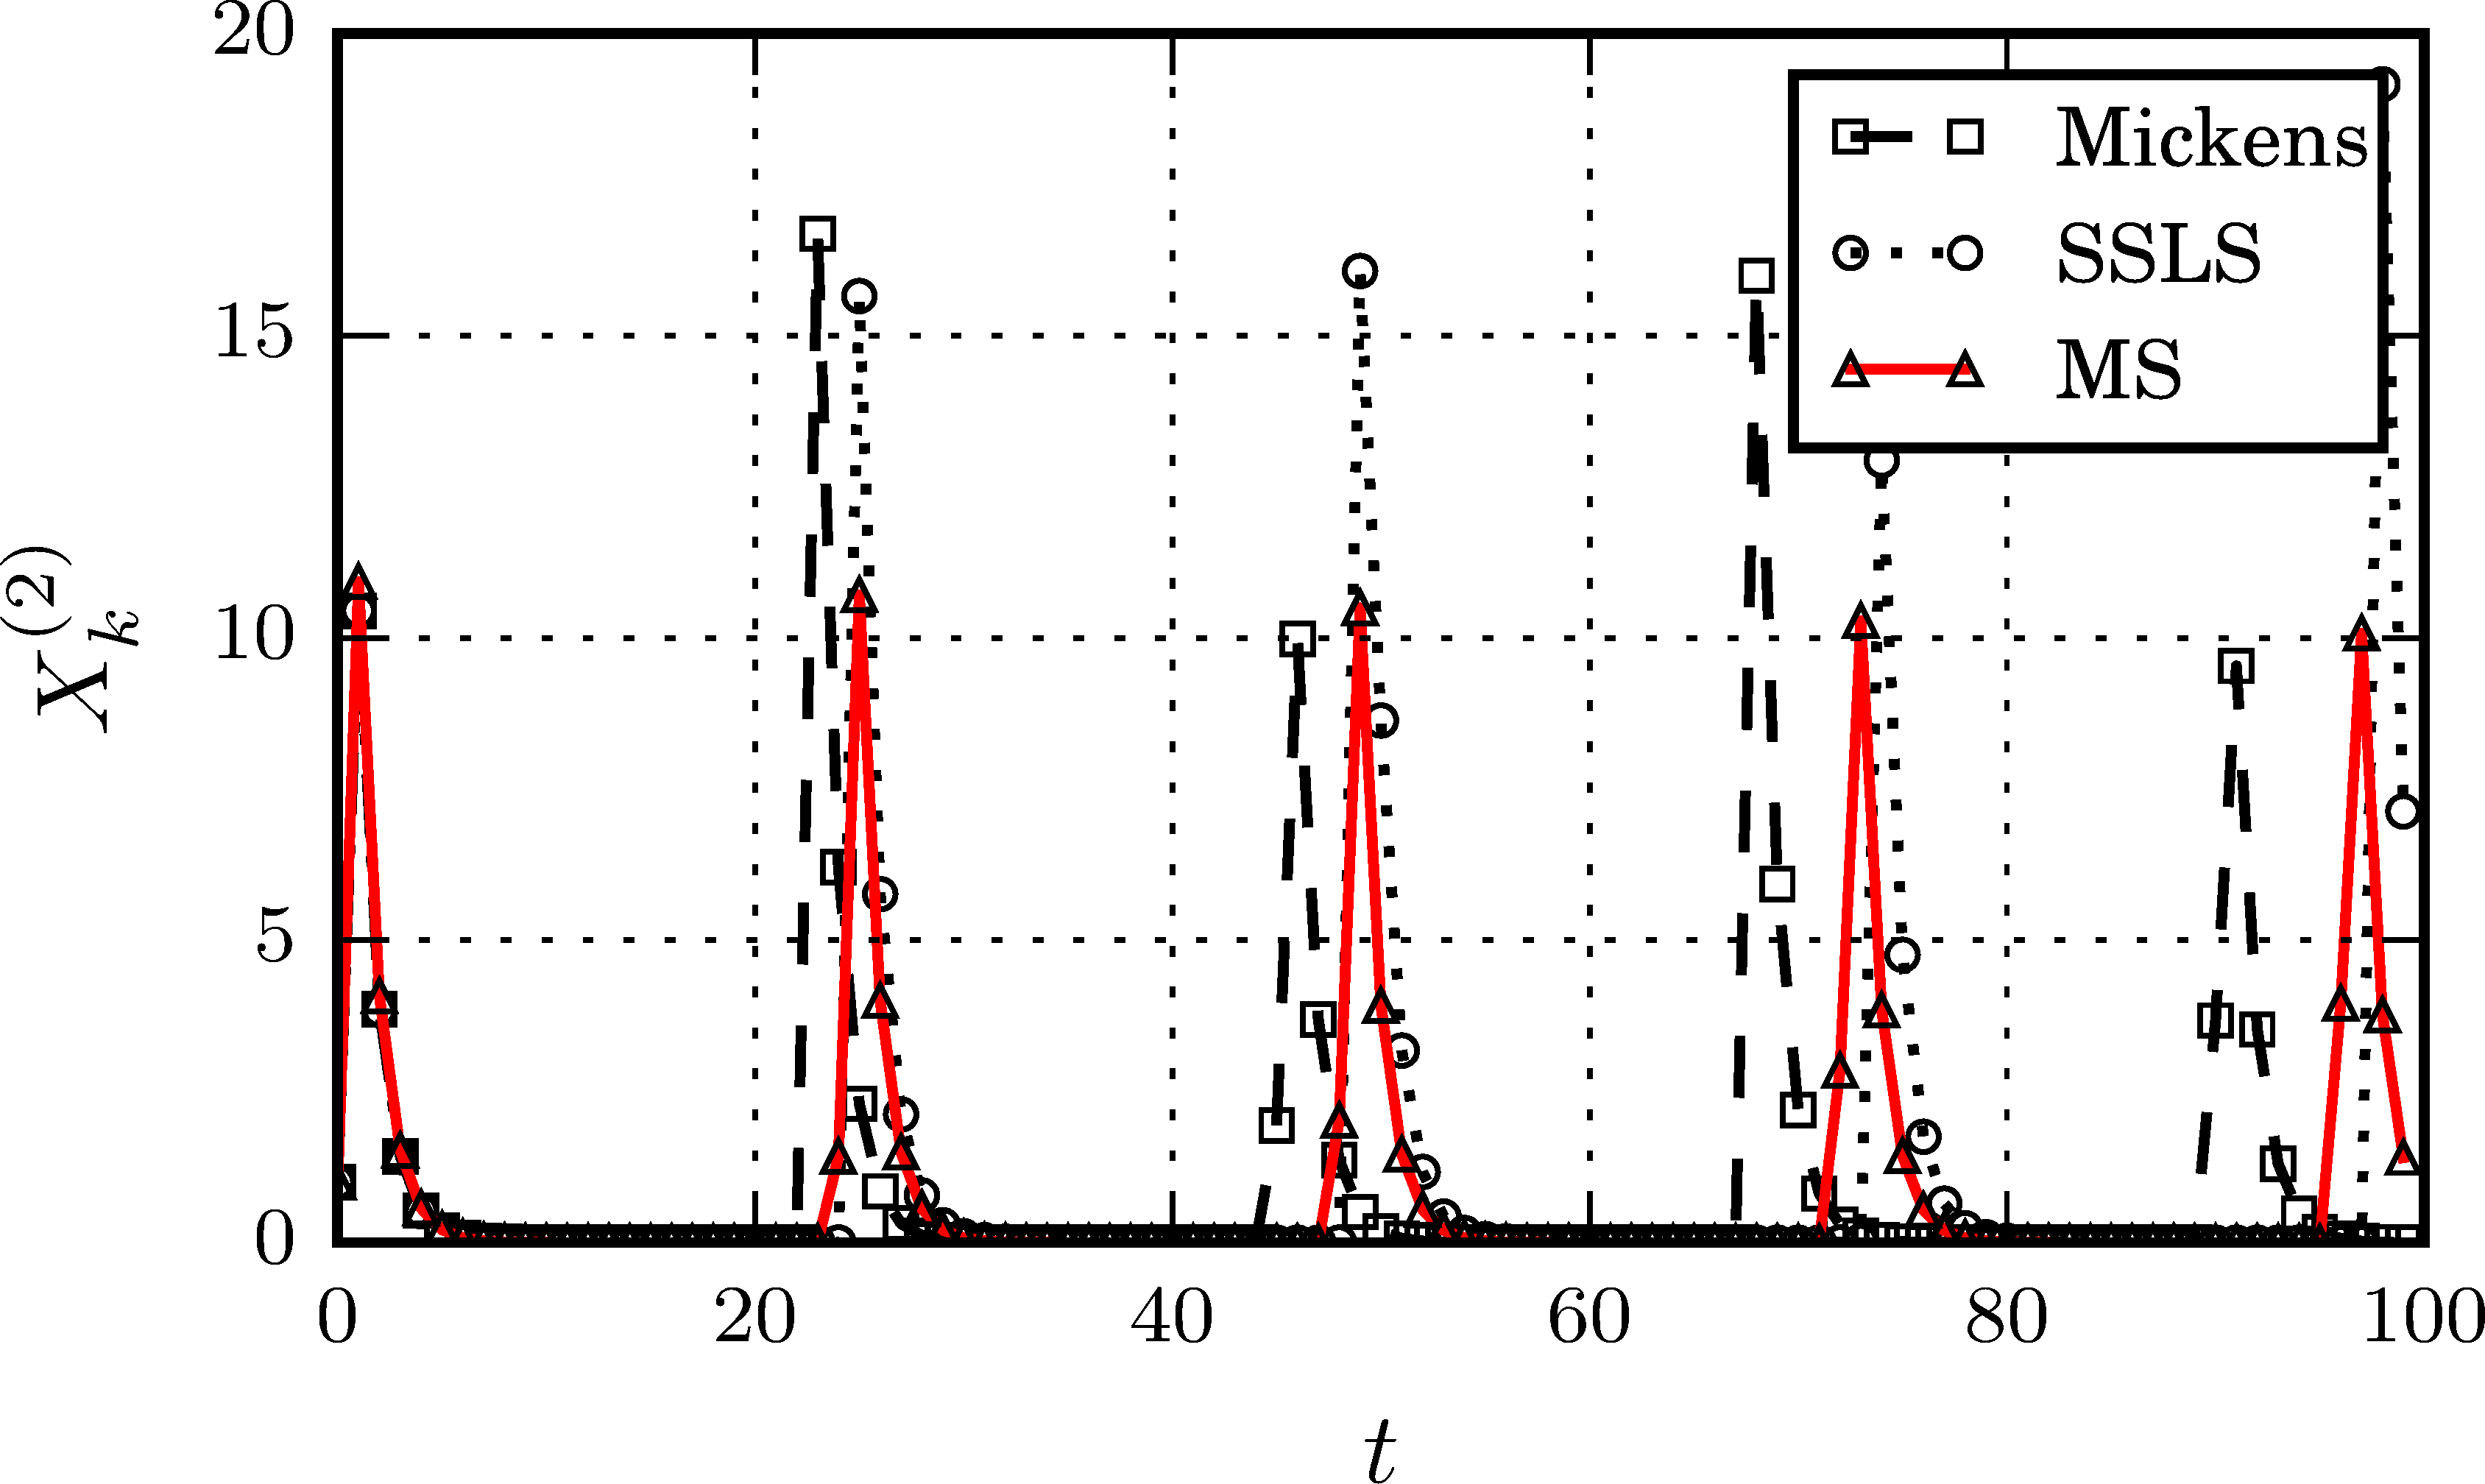
\includegraphics{./papers/paperB/figures/DetX2LotkaVolterraArnold.png}
		\label{subfig:DetX2LotkaVolterraArnold}
	}
	\caption{Likening between the deterministic schemes of Mickens, Serghini and LS for
		the Lotka-Volterra ODE 	\crefrange{eqn:DetLotkaVolterraArnoldA}{eqn:DetLotkaVolterraArnoldB} with 
		$a=1$,
		$b=1$,
		$c=1$,
		%$\sigma=0$,
		$(x_0^{(0)},y_0^{(1)})= (20.0,1.0).$
		$h=\num{.01}$, 
		and over the time interval $[0, 100]$.
	}\label{fig:DeterministicLotkaVolterra}
\end{figure}
\todo{change the legend label MS to Serghini.}
\begin{figure}[tb]
	\centering
	\subfloat[]{
		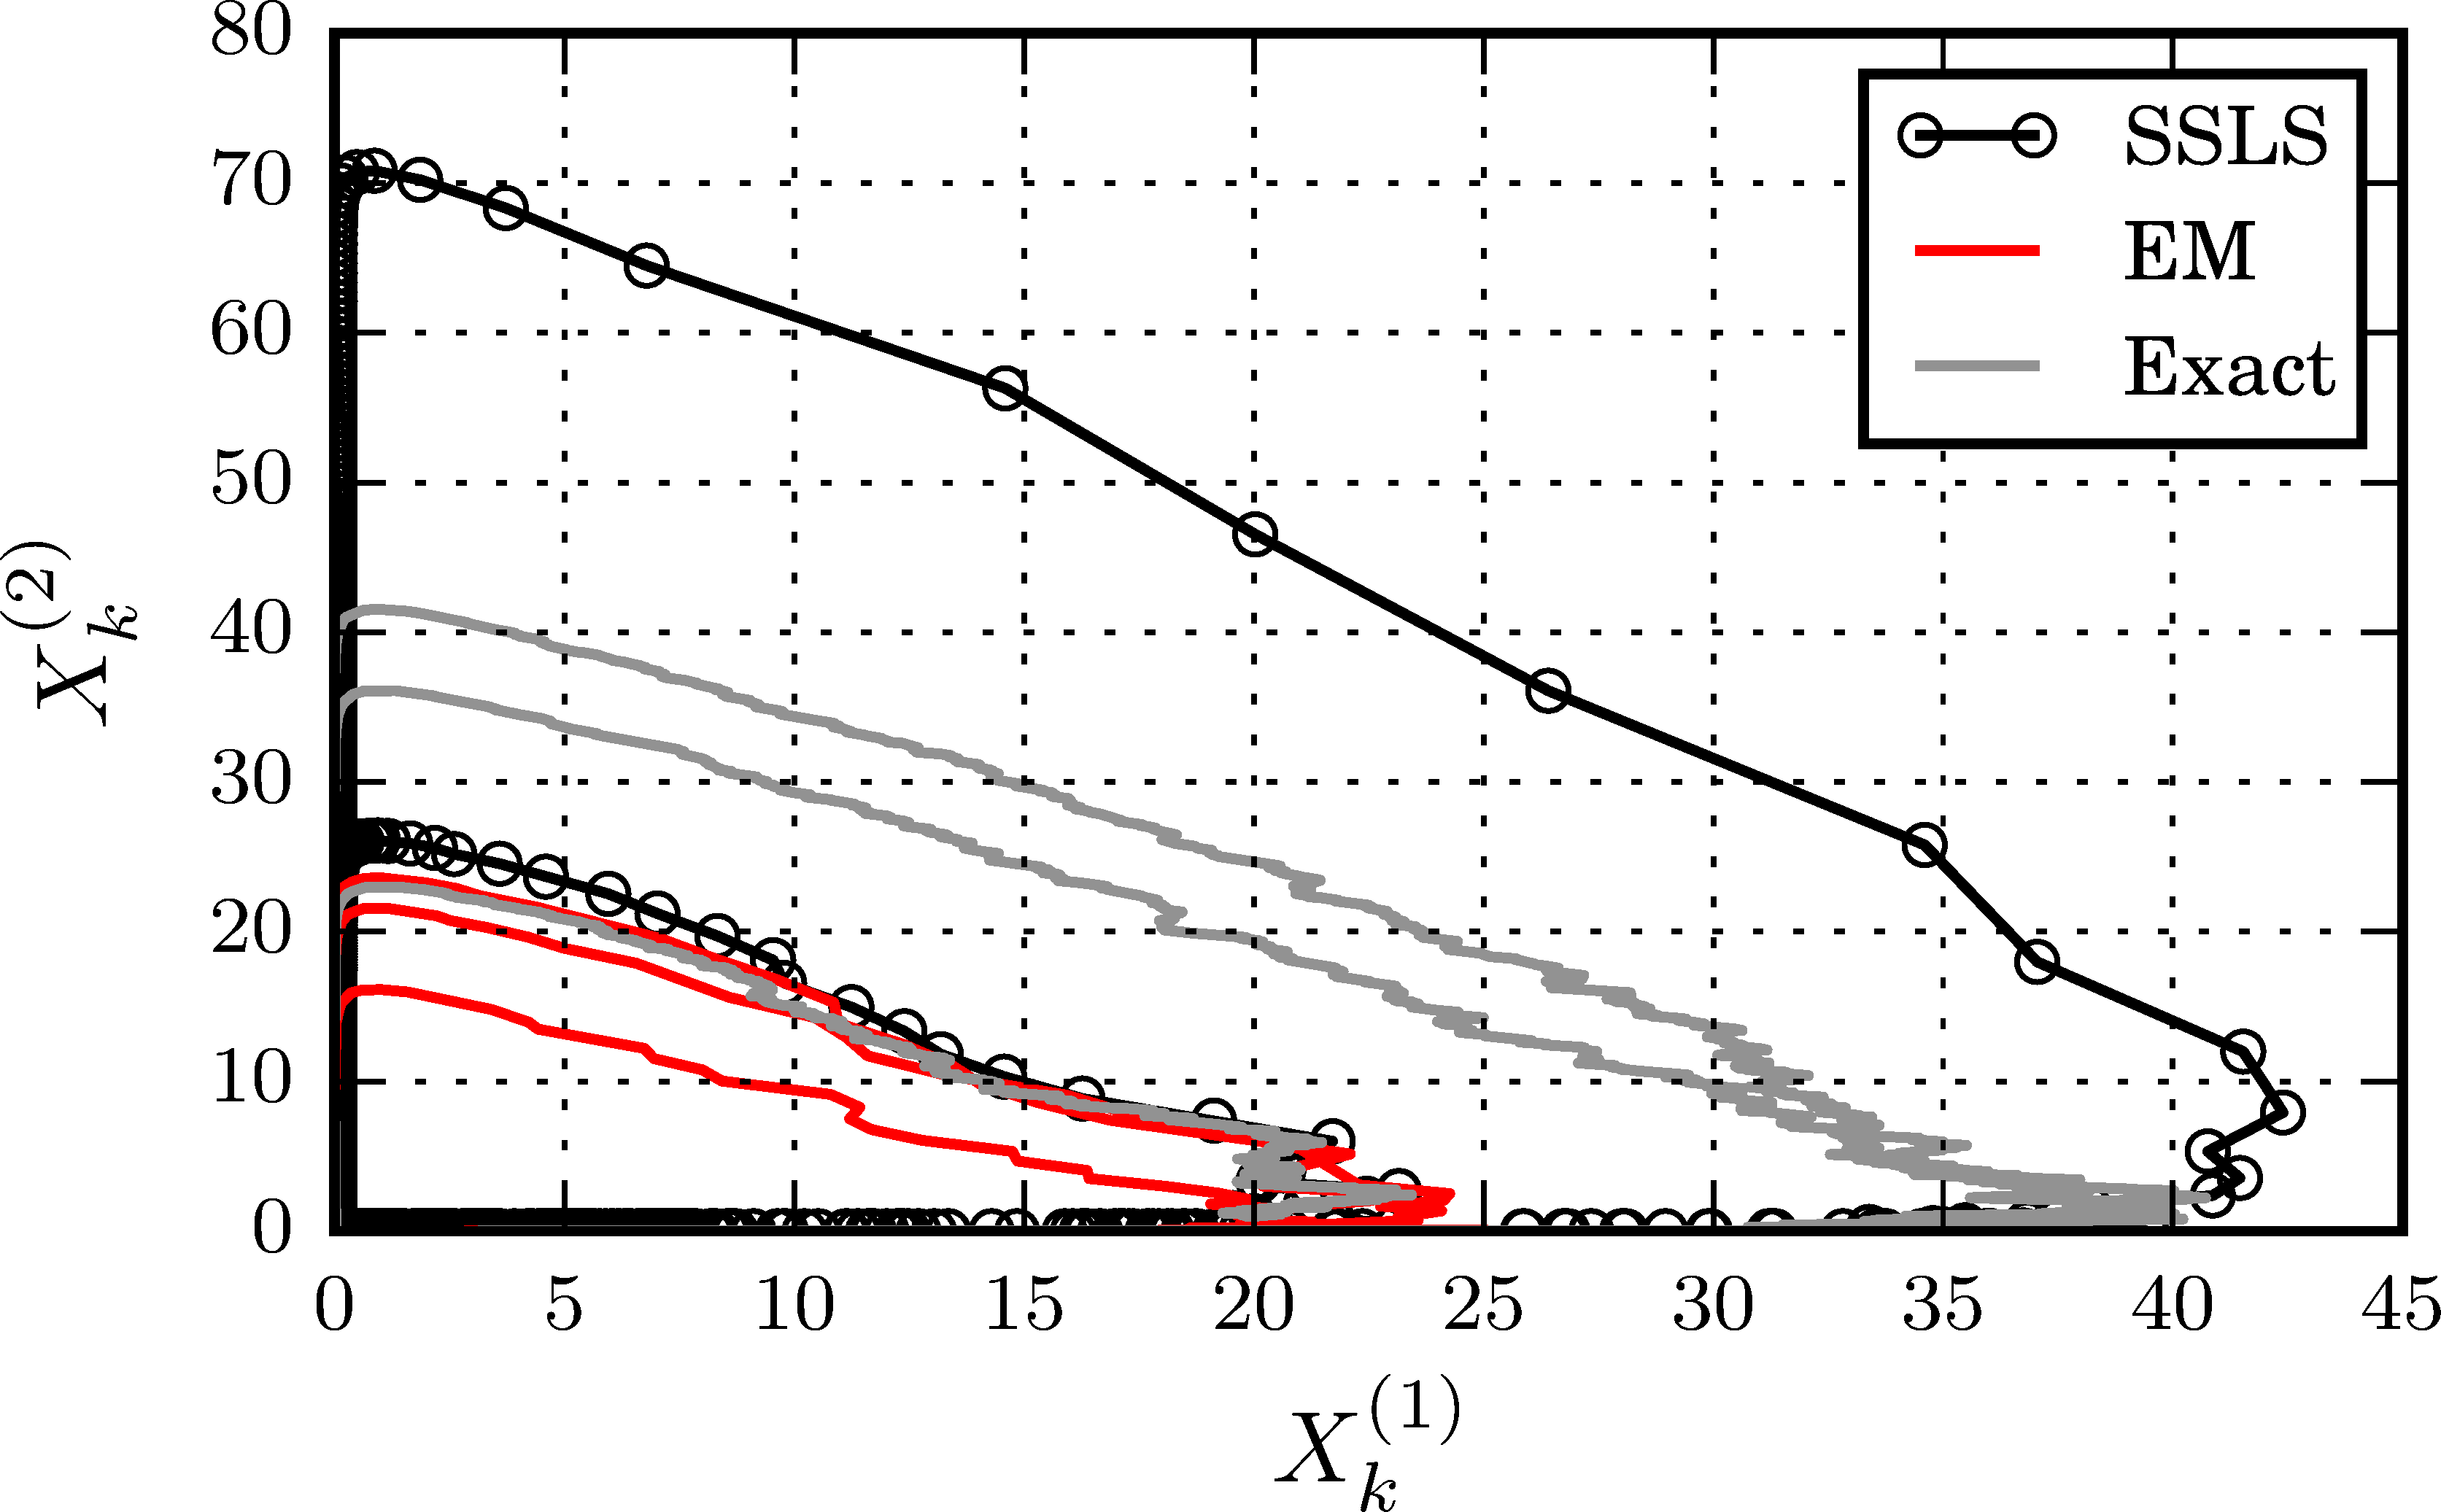
\includegraphics{./papers/paperB/figures/PhasePotraitLotkaVolterraArnold.png}
		\label{subfig:StoPhasePotraitLotkaVolterraArnold}
	}\\
	\subfloat[]{
		\centering
		\includegraphics{./papers/paperB/figures/X1LotkaVolterraArnold.png}
		\label{subfig:StoX1LotkaVolterraArnold}
	}
	\subfloat[]{
		\centering
		\includegraphics{./papers/paperB/figures/X2LotkaVolterraArnold.png}
		\label{subfig:StoX2LotkaVolterraArnold}
	}
	\caption{
		 Likening between the (EM) and  methods for the underlying SDE
		with 
		$a=1$,
		$b=1$,
		$d=1$,
		$\left(X^{1}(0), X^{2}(0)\right) = (20,1)$
		and multiplicative noise intensity $\sigma = \num{0.5}$.
		Here the path labeled with "Exact" means a EM simulation with $h=\num{1e-4}$.
	}\label{fig:LotkaVolterraSDE}
\end{figure}
%
\restoregeometry
\subsection{Environmental Brownian noise suppresses explosions in population dynamics}
	A very important work in stochastic population modeling is \cite{Mao2002}. Here, \citeauthor*{Mao2002}
prove that stochastic environmental noise suppresses the deterministic population explosion, linked to the following SDE
\begin{equation}
	\diag(y_1(t),\dots, y_d(t))
	\left[
	f(y(t))dt + g(y(t))dW(t)
	\right],
\end{equation}
In order to illustrate their results. \citeauthor{Mao2002} report the EM approximation of
\begin{align}
	dy_1(t) &=
		y_1(t) \left[1 - y_1(t) + 2 y_2(t) \right]dt + \varepsilon y_1^2(t) dW_1(t), \label{eqn:MaoPopDynSDE1}\\
	dy_2(t) &=
		y_2(t) \left[1 - 2 y_2(t) + 2 y_1(t)\right]dt + \varepsilon y_2^2(t) dW_2(t) \label{eqn:MaoPopDynSDE2}.
\end{align}
%

	To show that \SM method ()-() preserves this kind of behavior, we perform a numerical realization of this SDE.
In \Cref{fig:MaoPopDynSDE} using the EM and \SM discretizations,  we contrast the explosive deterministic nature of
\crefrange{eqn:MaoPopDynSDE1}{eqn:MaoPopDynSDE2} with its stochastic stabilization.
%
%\begin{align}
%	X_{k+1} &=	\frac{\exp(h a(Y_k)) X_k }{ a(Y_k) + X_k (\exp(h a(y_k)))}
%	\label{eqn:SteklovMatusSDELotka1}\\
%	Y_{k+1} &=	\frac{\exp(2 h b(X_{k+1})) Y_k }{ b(X_{k+1}) + 
%		Y_k( \exp(2h b( X_{k+1})))},
%		\label{eqn:SteklovMatusSDELotka2}
%\end{align}
%and the underlying linearized version \SM.
%
%
%\newgeometry{left=1.75cm, right=1.75cm}
\begin{figure}[h!]
%		\subfloat[]
%		{
%			\centering
%			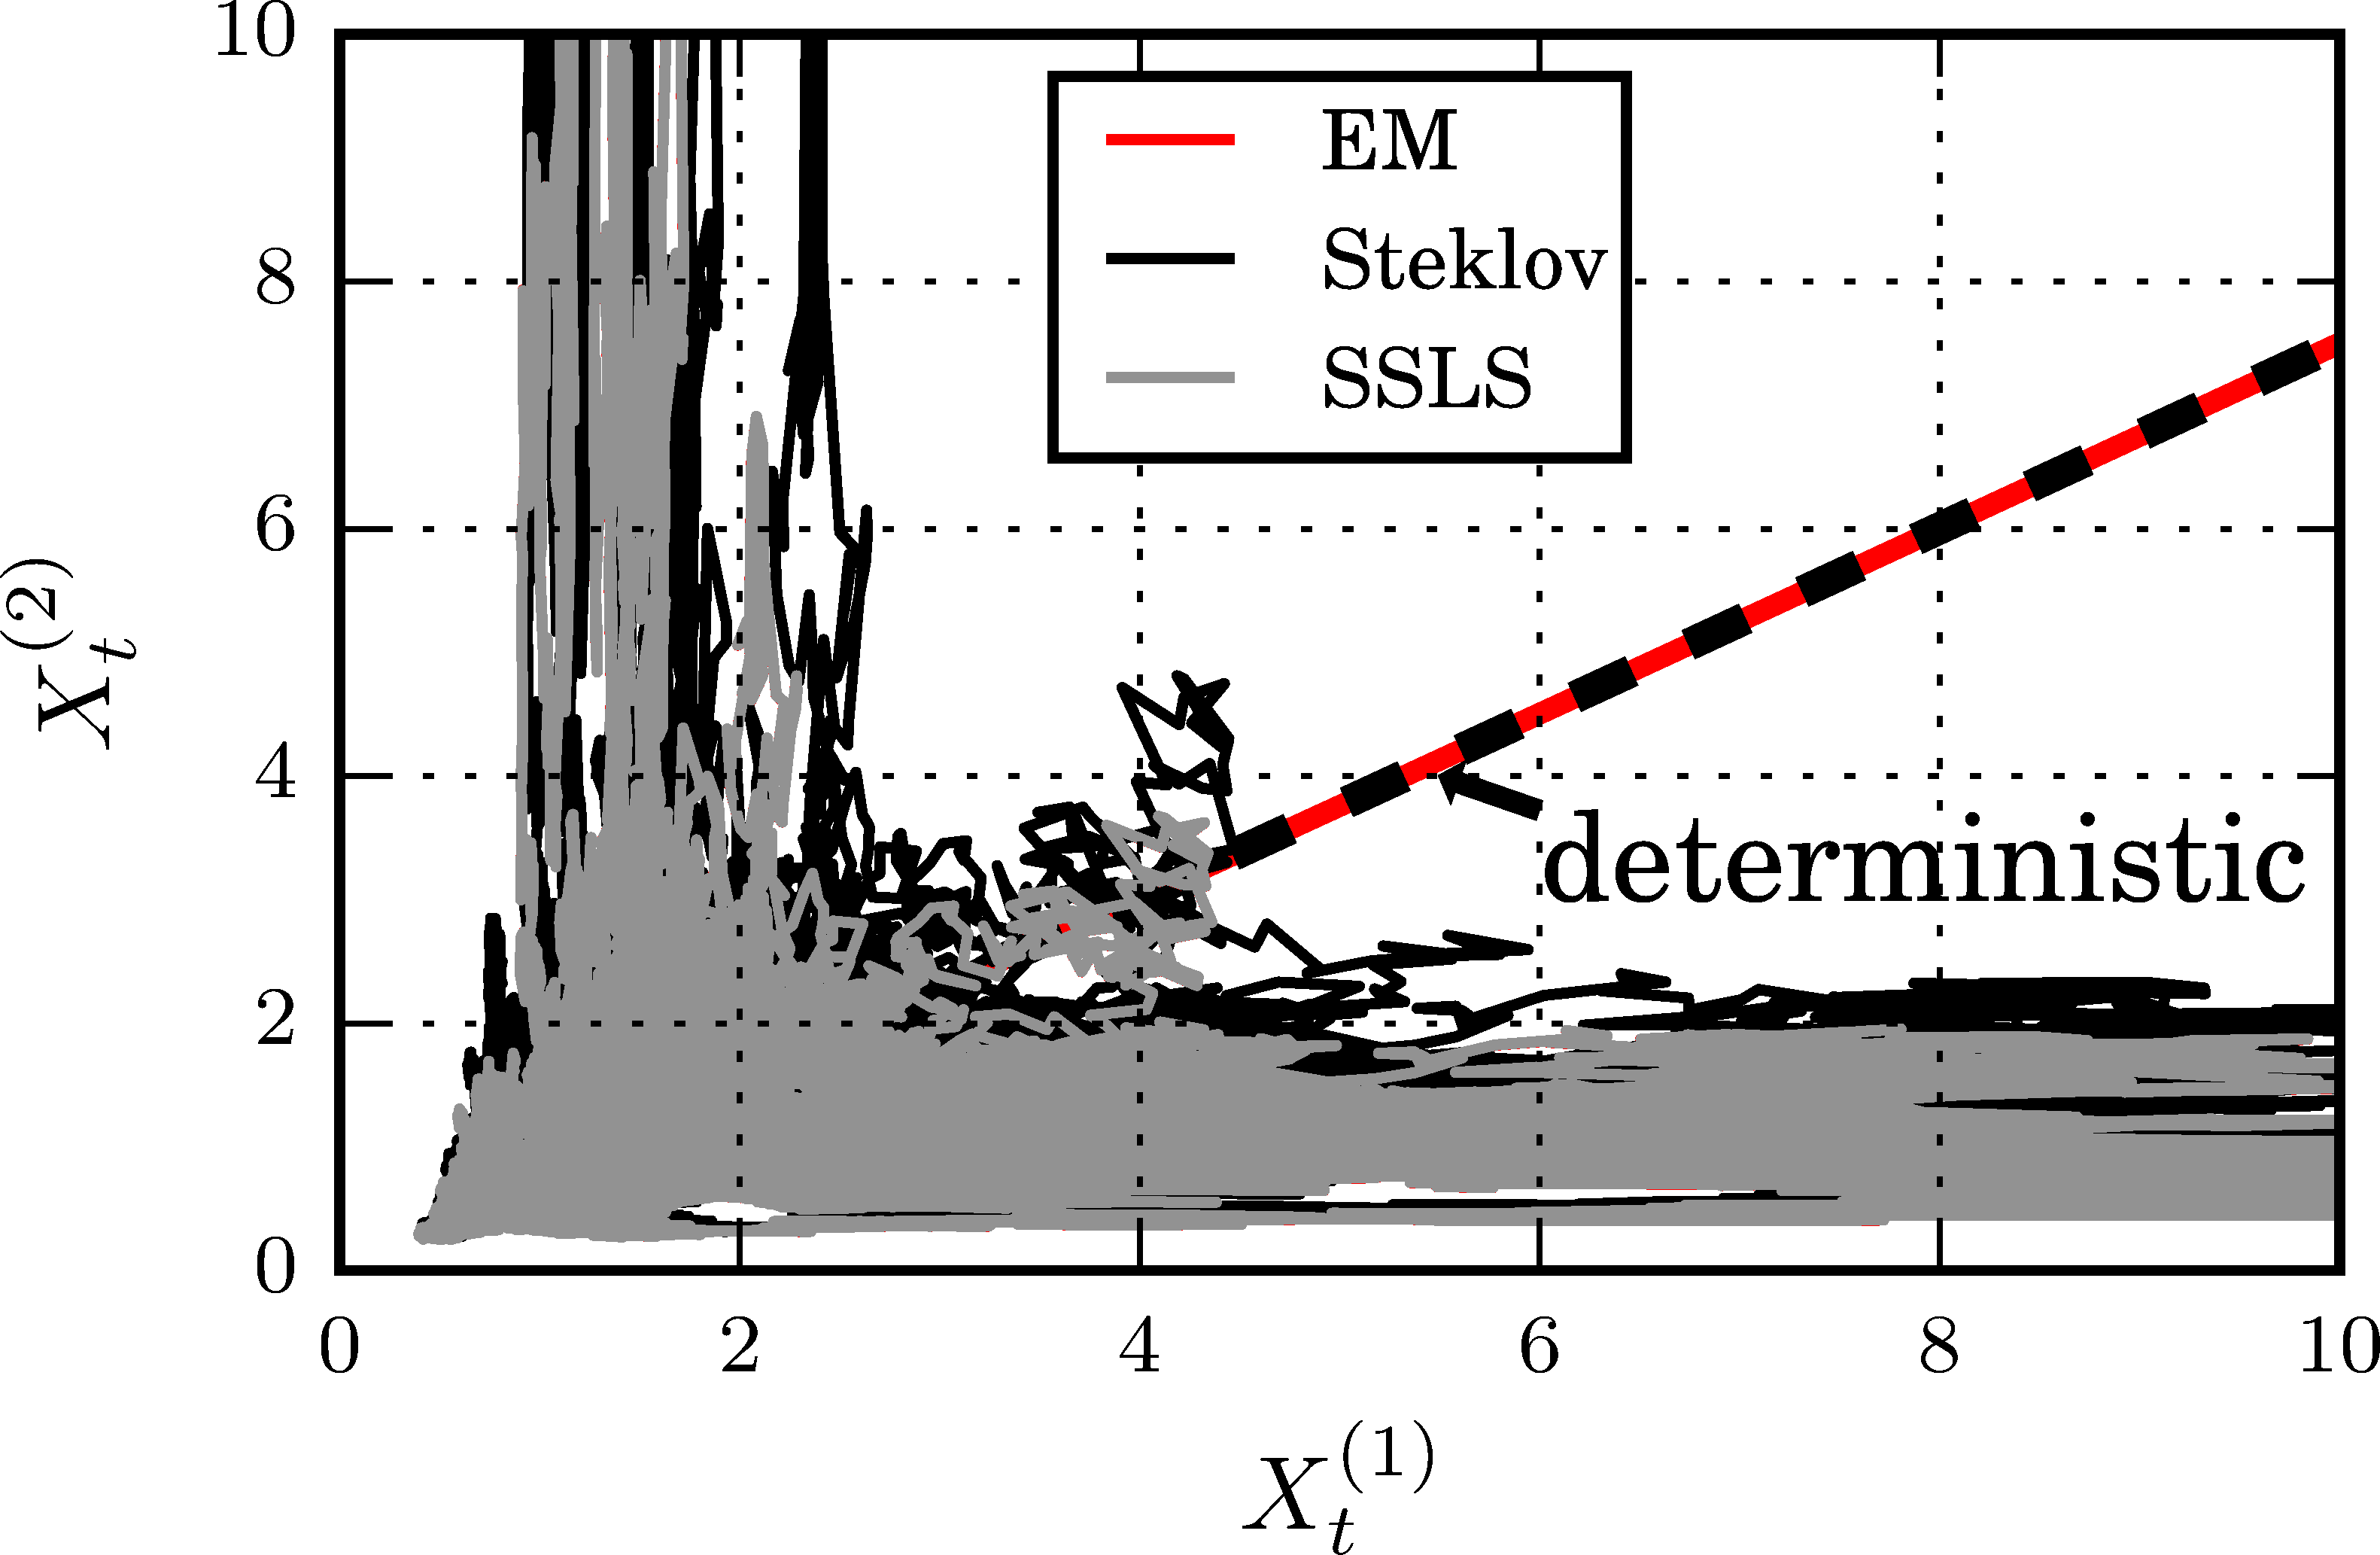
\includegraphics{./papers/paperB/figures/PhasePotraitMao}
%			\label{subfig:StoMaoPopDynPhasePotrait}
%		}\\
	\centering
	\subfloat[]
	{
		\includegraphics{./papers/paperB/figures/StoDetX1Mao}
		\label{subfig:subfig:StoMaoPopDynX1}
	}
	\subfloat[]
	{
		\centering
		\includegraphics{./papers/paperB/figures/StoDetX2Mao}
		\label{subfig:subfig:StoMaoPopDynX2}
	}
	\caption{
		Likening between the numerical solutions of SDE \crefrange{eqn:MaoPopDynSDE1}{eqn:MaoPopDynSDE2} 
		with the EM, Steklov and  \SM methods. We set the noise intensity at $\xi=1$ and fix the initial condition
		to $x(0)=(1, 1)$ over the time interval $T = [0, 10]$, and a step size $h=\num{1e-06}$.
	}
	\label{fig:MaoPopDynSDE}
\end{figure}

\todo{Fix the label into the legends}
\restoregeometry